\paragraph{}This chapter will give a brief introduction on how differential buffers and some theory behind it. The basic differential buffer can be built based in a fully differential operational transconductance amplifier (OTA). Most of CMOS integrated circuit make use of those types of amplifier, as they are easy to build and have many applications (as comparators, oscillators, peak detectors, etc). This type of amplifier is often proposed in literature because of its performance in respect to its linearity, output swing, supply voltage and its differential characteristic gives him a high resistance to some interferences such as external noise and to odd-order harmonics.(Apostila do baruqui)

\paragraph{}The basic idea is that those amplifiers have two differential inputs and outputs instead of the classic operation amplifier that has two single inputs, the inverting and non-inverting inputs, and one output. For the Fully Differential Amplifier (FDA), we have a differential non-inverting input and a differential inverting output, as shown in figure \ref{FDA}, and a fully differential output.

\begin{figure}
	\begin{center}
		\parbox[htb]{13.0cm}
		{
			\begin{center}
				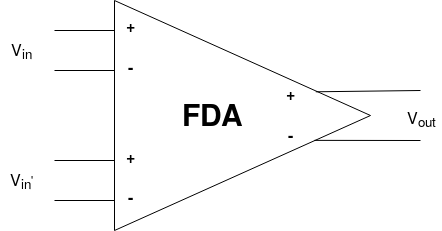
\includegraphics[scale=0.9]{FDA.png}
				\caption[\small{Fully diferential amplifier schematic.}]{\label{FDA} \small{Fully diferential amplifier schematic.}}
			\end{center}
		}
	\end{center}
\end{figure}

